%% LyX 2.0.6 created this file.  For more info, see http://www.lyx.org/.
%% Do not edit unless you really know what you are doing.
\documentclass{article}
\setlength{\parindent}{0cm}
\usepackage{array}
\usepackage{rotating}
\usepackage{fancybox}
\usepackage{calc}
\usepackage{multirow}
\usepackage{graphicx}

\makeatletter

%%%%%%%%%%%%%%%%%%%%%%%%%%%%%% LyX specific LaTeX commands.
%% Because html converters don't know tabularnewline
\providecommand{\tabularnewline}{\\}

%%%%%%%%%%%%%%%%%%%%%%%%%%%%%% Textclass specific LaTeX commands.
\newenvironment{lyxcode}
{\par\begin{list}{}{
\setlength{\rightmargin}{\leftmargin}
\setlength{\listparindent}{0pt}% needed for AMS classes
\raggedright
\setlength{\itemsep}{0pt}
\setlength{\parsep}{0pt}
\normalfont\ttfamily}%
 \item[]}
{\end{list}}

%%%%%%%%%%%%%%%%%%%%%%%%%%%%%% User specified LaTeX commands.
\usepackage{a4wide}

\makeatother

\begin{document}

\title{Matlab Visualization}


\date{University of Stuttgart, 2014}


\author{Jon Schlipf, Michael Mueller, Marc Gauger}

\maketitle
\newpage{}
\begin{abstract}
During our studies at the University of Stuttgart we created a Matlab
script to visualize the input of different Signals. This can be used
to verify a correct recording of a signal in an experimental environment
but can also be used to manipulate the signal to display it in different
ways.
\end{abstract}
\tableofcontents{}\newpage{}


\section{Introduction}

This software was created to analyze raw signal of all kinds but especially
radio frequency signals. It was developed at the University of Stuttgart
(Germany) during our studies. Therefore besides the authors the University
of Stuttgart is also part of the copyright holders. The script was
mainly developed for Matlab but can also be used under Octave. For
exceptions see \ref{sub:Exceptions-for-Octave}.


\subsection{Authors, License and Code}
\begin{itemize}
\item Michael Mueller (michael.mueller@sharkarea.net) 
\item Jon Schlipf (schlipf.jon@gmx.net)
\end{itemize}
Furthermore as supervising tutor: 
\begin{itemize}
\item Marc Gauger (Marc.Gauger@inue.uni-stuttgart.de) 
\end{itemize}
This program is distributed under the GPLv2 License which can be found
at 

\begin{center}
\textbf{http://www.gnu.org/licenses/gpl-2.0.html}
\par\end{center}

The Git Repository for this code can furthermore be accessed at 

\begin{center}
\textbf{https://github.com/ISharkI/matlab-visualization.git}
\par\end{center}


\subsection{Version}

Current (07/15/2014) Version of this program is 0.11. So far only
one single channel Signal is supported. 


\subsubsection{Changelog}
\begin{itemize}
\item 0.01 - Created the general structure and simple modules (Supervisor,
Loader, Delay Signal, simplePlot)
\item 0.02 - Created more modules (fourier, fourierBlocks, cutout, highpass,
lowpass, bandpass, energy spectrum, resampling, digital mixing)
\item 0.03 - Changed the interface between the modules
\item 0.04 - Created modules (correlation, plotIQ)
\item 0.1 - Added WebDemo for lessons
\item 0.11 - New versions of modules, new modules (findcorrelation, findsignal)
and a wifi-example
\end{itemize}
\newpage{}


\subsection{Exceptions for Octave\label{sub:Exceptions-for-Octave}}

Currently the following exceptions are known for ``not working''
under Octave below version 3.8 and without installed Octave-Forge
packages. (See \ref{sec:Available-Modules} for list of modules)
\begin{itemize}
\item PowerSpectrum
\item correlation
\item findCorrelation
\end{itemize}
\newpage{}


\section{Components}

The software consists of three parts as shown in Figure \ref{fig:Macro-structure-of}
\begin{itemize}
\item The ``Supervisor'' is the supervising engine and controls the combination
of the modules. It is the only part of this program which can be directly
accessed by the user.
\item The ``Loader'' are modules which convert the input to a usable format. 
\item The ``Modules'' are different modules (e.g. lowpass filter, simple
output) which can be consecutively added and walked through by the
supervisor. They are used to manipulate the signal or display it. 
\end{itemize}
\begin{figure}
\includegraphics[scale=0.3]{macrostructure}

\caption{Macro structure of the program\label{fig:Macro-structure-of}}


\end{figure}



\subsection{Supervisor}

Currently the supervisor is accessed by the following schema
\begin{lyxcode}
visualizeSignal(ModuleArray,~``inputFileLocation'',~{[}loaderModuleNumber{]},~{[}SampleRate{]})
\end{lyxcode}
In this schema the module array is an command array with an finite
number of filters (and their arguments) which the supervisor will
execute consecutiveley in a chain (See figure \ref{fig:Sequence}).
So it is just a list of commands which will passed to the modules
through the module interface later (See section \ref{sub:Modules}).

Therefore of course the array has N rows for N Modules. Each row consists
out of two parts
\begin{itemize}
\item The first element contains the module number (See section \ref{sec:Available-Modules})
\item The following elements contain the parameters for each module (See
section \ref{sec:Available-Modules} for the list). If no arguments
are needed or you need to fill the line up to get a complete array
it can be filled up with anything (e.g. zeroes). Parameters that are
not needed by the respective module will just be ignored.
\end{itemize}
Example:

\[
\left(\begin{array}{ccccc}
Module\, Number & Number\, of\, Parameters & Parameter\,1 & Parameter\,2 & ...\\
2 & 0 & 1 & 0 & 0\\
1 & 0 & 0 & 0 & 0\\
\ldots & \ldots & \ldots & \ldots & \ldots\\
4 & 1 & 0 & 0 & 0
\end{array}\right)
\]


By using the same interface for all module types (output, filter,
...), the user can display the output at any point in the module chain.\\


The ``loader module number'' is the number of the loader you want
to use (See section \ref{sub:Loader} and \ref{sec:Available-Loader}).
As the argument is optional the default is to load a Matlab file.
\\


Furthermore if no module array is given a ``{[}2 0 1{]}'' will be
assumed. This means the input is just displayed as a time plot without
modifications.

\begin{center}
\begin{figure}
\begin{centering}
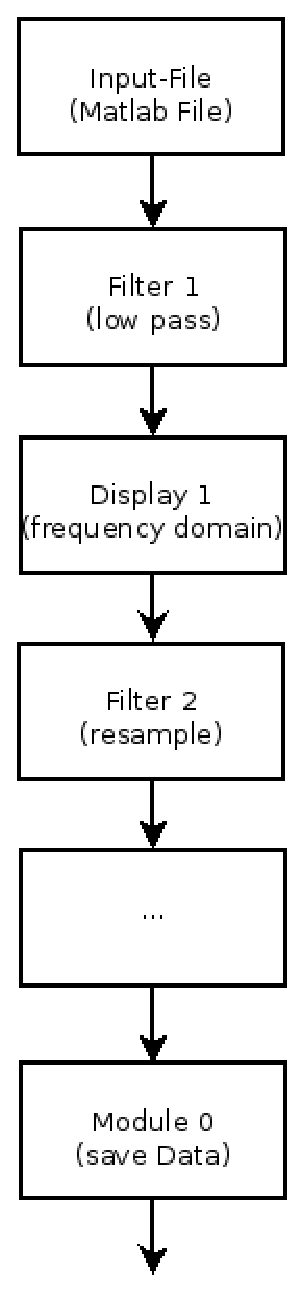
\includegraphics[scale=0.3]{sequence_full}
\par\end{centering}

\caption{Sequence of the program\label{fig:Sequence}}


\end{figure}

\par\end{center}


\subsection{Loader\label{sub:Loader}}

``Loader'' are modules used to import raw data for processing within
the supervisor. Each Loader is designed to import data from a specific
file type. They access the file through its file name and directory
path.

\newpage{}


\subsection{Modules\label{sub:Modules}}

The following modules are designed to perform different tasks but
are sharing a common interface. The Module Interface is an single
row array 

\[
\left(\begin{array}{ccc}
\left[N\right] & \left[P_{1}\ldots P_{N}\right]\left[SampleRate\right] & \left[\begin{array}{c}
ValueSignal\end{array}\right]\end{array}\right)
\]


Where 
\begin{itemize}
\item N - describes the amount of arguments passed to the module (second
row is filled with zero) 
\item $P_{1}\ldots P_{N}$ - are the arguments (While N is given in the
beginning of the array) 
\item SampleRate is the signal sample rate (time domain) or sample frequency
(frequency domain)
\item ValueSignal - are the signal values
\end{itemize}
This interface is used by the supervisor to call the modules and can
also be accessed manually for debug purposes. 

\newpage{}


\section{Available Loader\label{sec:Available-Loader}}


\subsection{loadMatlab\label{sub:loadMatlab}}

\shadowbox{\begin{minipage}[t]{1\columnwidth}%
\begin{itemize}
\item Name: \textbf{loadMatlab.m}
\item Loader number: \textbf{1}
\item Loads File Type: \textbf{{*}.mat}
\end{itemize}
\textbf{Function}: This Loader loads the raw signal from a Matlab
file which contains two vectors. It assumes ``v'' as the vector
with the discrete values for each ``t'' vector containing the corresponding
time values.%
\end{minipage}}


\subsection{loadCsv}

\shadowbox{\begin{minipage}[t]{1\columnwidth}%
\begin{itemize}
\item Name: \textbf{loadCsv.m}
\item Loader number: 2
\item Loads File Type: \textbf{{*}.csv}
\end{itemize}
\textbf{Function}: This Loader loads the signal from a CSV file which
contains the discrete values for each point of time. 

\textbf{Note}: If you use this Loader you need to give a sample rate
in the beginning.%
\end{minipage}}


\section{Available Modules\label{sec:Available-Modules}}

We differentiate between two kind of Modules:
\begin{itemize}
\item ``Modifier Modules'' are used to manipulate signals when the supervisor
calls them, its ``signal'' variable is overwritten and its old state
is lost. Modifier Modules can also change the way the signal is to
be interpreted. For example, the ``fourier'' module applies an fast
fourier transformation or inverse fast fourier transformation, thus
transforming the signal to another domain. This information will not
be saved, so the sequence of the modules is important.
\item ``Output Modules'' do not manipulate the signal, but display or
output its current state. 
\item Furthermore there is a ``Module'' to save your data (Module number
0 without arguments). So the last Plot and the last processed Signal
will be saved if you add an array of zeroes in between the modules.
Using this module it will generate an JPG, an FIG and a MAT File containing
the last plot and the current data.
\end{itemize}
\begin{table}
\begin{centering}
\begin{sideways}
\begin{tabular}{|l||l|l|l|l|l|}
\hline 
\textbf{Module} & \textbf{\#} & \textbf{Parameter 1} & \textbf{Parameter 2} & \textbf{Parameter 3} & \textbf{Parameter 4}\tabularnewline
\hline 
\hline 
saveData & 0 & - & - & - & -\tabularnewline
\hline 
\hline 
delayFilter & 1 & - & - & - & -\tabularnewline
\hline 
\hline 
\multirow{6}{*}{simplePlot} & \multirow{6}{*}{2} & \textbf{type:} & \multirow{6}{*}{figure number} & \multirow{6}{*}{-} & \multirow{6}{*}{-}\tabularnewline
\cline{3-3} 
 &  & 0 - time domain &  &  & \tabularnewline
\cline{3-3} 
 &  & 1 - frequency domain &  &  & \tabularnewline
\cline{3-3} 
 &  & 2 - phase in frequency &  &  & \tabularnewline
\cline{3-3} 
 &  & 3 - symmetric time &  &  & \tabularnewline
\cline{3-3} 
 &  & 4 - log. frequency &  &  & \tabularnewline
\hline 
\hline 
\multirow{3}{*}{fourier} & \multirow{3}{*}{3} & \textbf{type:} & \multirow{3}{*}{-} & \multirow{3}{*}{-} & \multirow{3}{*}{-}\tabularnewline
\cline{3-3} 
 &  & 0 - FFT &  &  & \tabularnewline
\cline{3-3} 
 &  & 1 - IFFT &  &  & \tabularnewline
\hline 
\hline 
fourierBlocks & 4 & length (samples) & - & - & -\tabularnewline
\hline 
\hline 
cutout & 5 & start sample & end sample & - & -\tabularnewline
\hline 
\hline 
\multirow{4}{*}{pass filter} & \multirow{4}{*}{6} & \textbf{type:} & \textbf{first frequency:} & \textbf{second frequency:} & \textbf{input domain:}\tabularnewline
\cline{3-6} 
 &  & 0 - low pass & limit for LP/HP & upper limit BP & 0 - time\tabularnewline
\cline{3-6} 
 &  & 1 - high pass & lower limit BP & \multirow{2}{*}{} & 1 - frequency\tabularnewline
\cline{3-4} \cline{6-6} 
 &  & 2 - band pass &  &  & \tabularnewline
\hline 
\hline 
powerSpectrum & 7 & - & - & - & -\tabularnewline
\hline 
\hline 
audioOutput & 8 & - & - & - & -\tabularnewline
\hline 
\hline 
resampling & 9 & P (interp. factor) & Q (dec. factor) & - & -\tabularnewline
\hline 
\hline 
\multirow{3}{*}{digitalMix} & \multirow{3}{*}{10} & \textbf{domain:} & \multirow{3}{*}{frequency (Hz)} & \multirow{3}{*}{-} & \multirow{3}{*}{-}\tabularnewline
\cline{3-3} 
 &  & 0 - time &  &  & \tabularnewline
\cline{3-3} 
 &  & 1 - frequency &  &  & \tabularnewline
\hline 
\hline 
\multirow{5}{*}{correlation} & \multirow{5}{*}{11} & \textbf{target signal:} & \multirow{5}{*}{-} & \multirow{5}{*}{-} & \multirow{5}{*}{-}\tabularnewline
\cline{3-3} 
 &  & 0 - autocorrelate &  &  & \tabularnewline
\cline{3-3} 
 &  & 1 - 802.11g short &  &  & \tabularnewline
\cline{3-3} 
 &  & 2 - 802.11g long &  &  & \tabularnewline
\cline{3-3} 
 &  & 3 - loading prompt &  &  & \tabularnewline
\hline 
\hline 
plotIQ & 12 & - & - & - & -\tabularnewline
\hline 
\hline 
findSignal & 13 & - & - & - & -\tabularnewline
\hline 
\hline 
\multirow{5}{*}{findCorrelation} & \multirow{5}{*}{14} & \textbf{target signal:} & \multirow{5}{*}{-} & \multirow{5}{*}{-} & \multirow{5}{*}{-}\tabularnewline
\cline{3-3} 
 &  & 0 - autocorrelate &  &  & \tabularnewline
\cline{3-3} 
 &  & 1 - 802.11g short &  &  & \tabularnewline
\cline{3-3} 
 &  & 2 - 802.11g long &  &  & \tabularnewline
\cline{3-3} 
 &  & 3 - loading prompt &  &  & \tabularnewline
\hline 
\end{tabular}
\end{sideways}
\par\end{centering}

\caption{Short reference for module array usage}


\end{table}


\newpage{}


\subsection{delayFilter}

\shadowbox{\begin{minipage}[t]{1\columnwidth}%
\begin{itemize}
\item Name: \textbf{delayFilter.m}
\item Module number: \textbf{1}
\item Module type: \textbf{Modifier}
\item Arguments: 0
\item Function: Does nothing and may be used to wait for other processes/signals
etc.\end{itemize}
%
\end{minipage}}


\subsection{simplePlot}

\shadowbox{\begin{minipage}[t]{1\columnwidth}%
\begin{itemize}
\item Name: \textbf{simplePlot.m}
\item Module number: 2
\item Module type: \textbf{Output}
\item Arguments: 3

\begin{itemize}
\item first argument: type

\begin{itemize}
\item determines how the signal should be plottet
\item possible values:

\begin{itemize}
\item 0 - time domain
\item 1 - frequency domain
\item 2 - phase in frequency domain
\item 3 - symmetric time domain
\item 4 - logarithmic frequency domain
\end{itemize}
\end{itemize}
\item second argument: figure number - determines in which figure number
the signal is to be plotted 
\item third argument: sample rate (is automatically handed over by the supervisor
and does not need to be part of the command array)
\end{itemize}
\item Function: Plots a signal in the requested figure. It depends on the
argument 'type' how the signal should be plotted.\end{itemize}
%
\end{minipage}}


\subsection{fourier}

\shadowbox{\begin{minipage}[t]{1\columnwidth}%
\begin{itemize}
\item Name: \textbf{fourier.m}
\item Module number: 3
\item Module type: \textbf{Modifier}
\item Arguments: 2

\begin{itemize}
\item first argument: type

\begin{itemize}
\item determines what kind of transformation should be done
\item possible values:

\begin{itemize}
\item 0 - fast fourier transform
\item 1 - inverse fast fourier transform
\end{itemize}
\end{itemize}
\item second argument: sample rate/dist (is automatically handed over by
the supervisor and does not need to be part of the command array)
\end{itemize}
\item Function: Applies a fast fourier transform or an inverse fast fourier
transform, depending on the argument ``type''.\end{itemize}
%
\end{minipage}}


\subsection{fourierBlocks}

\shadowbox{\begin{minipage}[t]{1\columnwidth}%
\begin{itemize}
\item Name: \textbf{fourierBlocks.m}
\item Module number: \textbf{4}
\item Module type: \textbf{Modifier}
\item Arguments: 2

\begin{itemize}
\item first argument: block length

\begin{itemize}
\item {[}1:duration of signal{]} determines the length (in samples) of the
blocks the signal will be divided into
\end{itemize}
\item second argument: sample rate/dist (is automatically handed over by
the supervisor and does not need to be part of the command array)
\end{itemize}
\item Function: Displays a three dimensional (time-dependent) spectrum.\end{itemize}
%
\end{minipage}}


\subsection{cutout}

\shadowbox{\begin{minipage}[t]{1\columnwidth}%
\begin{itemize}
\item Name: \textbf{cutout.m}
\item Module number: \textbf{5}
\item Module type: \textbf{Modifier}
\item Arguments: 2

\begin{itemize}
\item first argument: start sample

\begin{itemize}
\item {[}1:startsample{]} determines the start sample of the signal which
will be cut out
\end{itemize}
\item second argument: end sample

\begin{itemize}
\item {[}1:endsample{]} determines the end sample of the signal which will
be cut out
\end{itemize}
\end{itemize}
\item Function: If ``startsample'' is smaller than ``endsample'', all
samples between the two samples will be returned. If ``startsample''
is greater than ``endsample'', the function returns the samples
between startsample and the end of the input signal and the samples
between the beginning and endsample. If the two arguments are equal,
the sample at that position will be returned.\end{itemize}
%
\end{minipage}}


\subsection{passFilter}

\shadowbox{\begin{minipage}[t]{1\columnwidth}%
\begin{itemize}
\item Name: \textbf{passFilter.m}
\item Module number: \textbf{6}
\item Module type: \textbf{Modifier}
\item Arguments: 5

\begin{itemize}
\item first argument: type of filter

\begin{itemize}
\item 0 - lowpass
\item 1 - highpass
\item 2 - bandpass
\end{itemize}
\item second argument: first frequency

\begin{itemize}
\item limit frequency for low- or highpass, lower limit frequency for bandpass
\end{itemize}
\item third argument: second frequency

\begin{itemize}
\item higher limit frequency for bandpass (ignored for low- or highpass)
\end{itemize}
\item fourth argument: domain

\begin{itemize}
\item 0 - input signal is in time domain
\item 1 - input signal is in frequency domain
\end{itemize}
\item fifth argument: sample rate/dist (is automatically handed over by
the supervisor and does not need to be part of the command array)
\end{itemize}
\item Function: Applies a pass filter to the signal \end{itemize}
%
\end{minipage}}


\subsection{powerSpectrum}

\shadowbox{\begin{minipage}[t]{1\columnwidth}%
\begin{itemize}
\item Name: \textbf{powerSpectrum.m}
\item Module number: \textbf{7}
\item Module type: \textbf{Output}
\item Arguments: 1

\begin{itemize}
\item first argument: sample rate (is automatically handed over by the supervisor
and does not need to be part of the command array)
\end{itemize}
\item Function: Provides the power spectrum as data in return and also displays
it
\end{itemize}
\textbf{Note:} This Module will not work with Octave below version
3.8 and installed Octave-Forge packages.%
\end{minipage}}


\subsection{audioOutput}

\shadowbox{\begin{minipage}[t]{1\columnwidth}%
\begin{itemize}
\item Name: \textbf{audioOutput.m}
\item Module number: \textbf{8}
\item Module type: \textbf{Output}
\item Arguments: 1

\begin{itemize}
\item first argument: sample rate (is automatically handed over by the supervisor
and does not need to be part of the command array)
\end{itemize}
\item Function: Outputs the signal using the matlab function ``sound''
at the PC speaker with the given sample rate (or at least tries to)\end{itemize}
%
\end{minipage}}


\subsection{resampling}

\shadowbox{\begin{minipage}[t]{1\columnwidth}%
\begin{itemize}
\item Name: \textbf{resampling.m}
\item Module number: \textbf{9}
\item Module type: \textbf{Modifier}
\item Arguments: 3

\begin{itemize}
\item first argument: P (interpolation factor)
\item second argument: Q (decimation factor)
\item third argument: sample rate (is automatically handed over by the supervisor
and does not need to be part of the command array)
\end{itemize}
\item Function: resamples the signal by the given factors\end{itemize}
%
\end{minipage}}


\subsection{digitalMix}

\shadowbox{\begin{minipage}[t]{1\columnwidth}%
\begin{itemize}
\item Name: \textbf{digitalMix.m}
\item Module number: \textbf{10}
\item Module type: \textbf{Modifier}
\item Arguments: 3

\begin{itemize}
\item first argument: domain

\begin{itemize}
\item 0 - timedomain
\item 1 - frequencydomain
\end{itemize}
\item second argument: value (frequency which is used to mix in Hz)
\item third argument: sample rate/dist (is automatically handed over by
the supervisor and does not need to be part of the command array)
\end{itemize}
\item Function: Mixes the signals\end{itemize}
%
\end{minipage}}


\subsection{correlation}

\shadowbox{\begin{minipage}[t]{1\columnwidth}%
\begin{itemize}
\item Name: \textbf{correlation.m}
\item Module number: \textbf{11}
\item Module type: \textbf{Modifier}
\item Arguments: 1

\begin{itemize}
\item target signal to correlate

\begin{itemize}
\item 0 - autocorrelation
\item 1 - 802.11g short sequence
\item 2 - 802.11g long sequence
\item 3 - gives a prompt to load a matlab file (See \ref{sub:loadMatlab})
\end{itemize}
\end{itemize}
\item Function: Correlates two signals with each other
\end{itemize}
\textbf{Note:} This Module will not work with Octave below version
3.8 and installed Octave-Forge packages.%
\end{minipage}}


\subsection{plotIQ}

\shadowbox{\begin{minipage}[t]{1\columnwidth}%
\begin{itemize}
\item Name: \textbf{plotIQ.m}
\item Module number: \textbf{12}
\item Module type: \textbf{Output}
\item Arguments: 0
\item Function: Generates an IQ-Plot of the given signal.\end{itemize}
%
\end{minipage}}


\subsection{findSignal}

\shadowbox{\begin{minipage}[t]{1\columnwidth}%
\begin{itemize}
\item Name: \textbf{findSignal.m}
\item Module number: \textbf{13}
\item Module type: \textbf{Modifier}
\item Arguments: 0
\item Function: Tries to find a wireless signal\end{itemize}
%
\end{minipage}}


\subsection{findCorrelation}

\shadowbox{\begin{minipage}[t]{1\columnwidth}%
\begin{itemize}
\item Name: \textbf{findCorrelation.m}
\item Module number: \textbf{14}
\item Module type: \textbf{Modifier}
\item Arguments: 1

\begin{itemize}
\item target signal to correlate

\begin{itemize}
\item 0 - autocorrelation
\item 1 - 802.11g short sequence
\item 2 - 802.11g long sequence
\item 3 - gives a prompt to load a matlab file (See \ref{sub:loadMatlab})
\end{itemize}
\end{itemize}
\item Function: Tries to find the correlation of both signal
\end{itemize}
\textbf{Note:} This Module will not work with Octave below version
3.8 and installed Octave-Forge packages.%
\end{minipage}}

\newpage{}


\section{Interface for Lessons}

We also created an interface (``webdemo'') for lessons so the programm
can be used in a ``quick and easy'' access. It is located at

\begin{center}
\textbf{http://webdemo.inue.uni-stuttgart.de/webdemos\_mgauger/06\_teamarbeit/visualizeSignal/index.php}
\par\end{center}

For this webdemo we simplified the program to fit it into the interface
and created a connection between the demo and the main program. The
User is only capable of adding a mixture of given filters though the
demo. Furthermore we added the possibility to upload your own signal
or use a predefined signal. 

Restrictions for the file upload are:
\begin{itemize}
\item Samplerate is known
\item CSV-File
\item File is not larger than 2MB
\end{itemize}
Using the complete program you would be able to apply hundreds of
filters after each other, save the states as files or display more
than one plot at a time. To keep it simple we reduced it to the following
filters
\begin{itemize}
\item Pass-Filter (Low-/High-/Bandpass)
\item Digital Mixing
\end{itemize}
Possible predefined signals to chose are: 
\begin{itemize}
\item An Wireless Signal (Channel 1)
\end{itemize}
For output you can choose between:
\begin{itemize}
\item time domain
\item frequency domain
\end{itemize}

\subsection{Usage}
\begin{enumerate}
\item Decide if you want to get the output as time or frequency domain or
as IQ demodulation
\item Decide if you want to use a predefined signal. If yes, keep the box
checked and choose from the dropdown. If you want to use your own
signal, remove the checked box and get ``Choose File'' to get a
file from your own PC. Please note: You need to know the samplerate
and the CSV-File is not larger than 2MB.
\item Check the filters you want to use

\begin{enumerate}
\item Pass-Filter


If you want to use a Pass-Filter chose which one you want to use.
Insert the border frequencies into the boxes in Hz.

\item Digital Mixing


If you want to mix your signal with an known frequency insert it in
Hz.

\end{enumerate}
\end{enumerate}
\newpage{}


\section{Possible future extension}

Of course one possible extension is the addition of other filters/modules.

Other possibilities (which cam to our mind while working on this program
but we had no time to do it)
\begin{itemize}
\item branches
\item conditions
\item live input using oszilloscopes (e.g. Picoscope)
\item If the Webdemo Server is upgraded to Octave 3.8 or above there are
several new modules possible for the webdemo\end{itemize}

\end{document}
